\documentclass[a4paper,12pt]{article}
\usepackage{../../mypackages}
\usepackage{../../macros}


\begin{document}

\title{Chapitre 4 : L'atome}
\author{N. Bancel}
\date{Octobre 2024}
\maketitle

\section{Exercices}

\subsection{Alcool}


\begin{figure}[H]
  \centering
  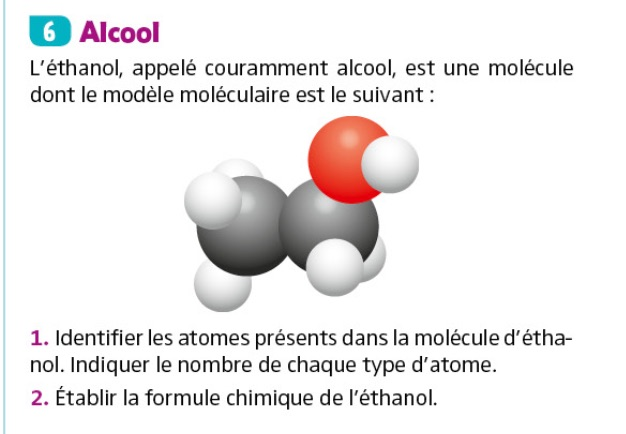
\includegraphics[width=0.7\linewidth]{ethanol.jpg}
\end{figure}

\subsection{Test de connaissances}


\begin{figure}[H]
  \centering
  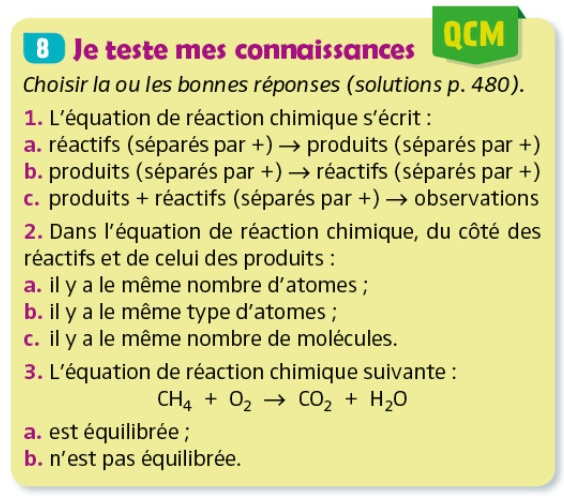
\includegraphics[width=0.7\linewidth]{test.jpg}
\end{figure}

\subsection{La rouille}

La formation de la rouill provient d'une réaction chimique entre le fer et le dioxygène de l'air.

\begin{enumerate}

 \item Ecrire l'équation de réaction chimique en toutes lettres
 \item Parmi les équations de réaction de formation de la rouille ci-dessous, identifier celle qui est équilibrée 
 
 \begin{itemize}[noitemsep]
  \item[A] \ce{Fe + O2 -> Fe2O3}
  \item[B] \ce{2 Fe + 3 O2 -> Fe2O3}
  \item[C] \ce{4 Fe + 3 O2 -> 2 Fe2O3}
 \end{itemize}

\end{enumerate}

\subsection{Photosynthèse}

Un élève de biologie a écrit l'équation de la photosynthèse (la transformation chimique à la base de la croissance des plantes), de la façon suivante : \par 
\[
\ce{6CO2 + 6H2O -> C6H12O6 + 6O2}
\]
 
\begin{itemize}[noitemsep]
  \item[1] Identifier les réactions et les produits. Les nommer. \ce{C6H12O6} est la molécule du sucre
  \item[2] Cette équation est-elle équilibrée ? 
 \end{itemize}


\end{document}
